\section{Evaluation}

  The present section aims at evaluating on a COTS platform the benefits brought by SchIM (w.r.t. memory isolation) and to demonstrate the good behaviour of the different embedded policies.
  %Therefore, we have integrated the SchIM IP on the PL side of a Xilinx ZCU102 development board, featuring a Xilinx Zynq UlraScale+ XCZU9EG SoC.
  %\todo[inline]{RM: move all the platform detailes to the impl. section}
  
  The present section is organised as follows. Firstly, in subsection \ref{subsection:considered-architecture}, the exact SchIM configuration on the ZCU102 development board is discussed. Thereafter, a full assessment of the board capabilities with and without SchIM is provided in subsection \ref{subsec:platform-capabilities-and-performance-degradation}. In subsection \ref{subsec:internal-behaviour-of-schim}, an analysis of the SchIM module behaviour is presented. Finally, a demonstration of the memory isolation enabled by SchIM using real benchmark applications is provided.

\todo[inline]{RM: Add an experimental setup subsection to describe:
  benchmarks, different routes that will be tests, parameters of the schedulers }
  
  \subsection{Experimental Setup}
    \label{subsection:considered-architecture}
    For this set of experiemtns, \schim has been evaluated by using synthetic benchmarks (or \emph{Memory Bombs}), real benchmarks issued from the San Diego Vision Benchmark Suite (SD-VBS) \cite{SD-VBS} (more specifically, the most \emph{Memory Bound} ones, deemed as \emph{VGA}) and combinations of the two.
%  \todo[inline]{RM: this part is a bit redundant with the implementation section. We can remove this seciton and only keep the description of the routes we are gonna test. See above}
%    The COTS platform used for the following set of experiments, the Xilinx ZCU102 development board, features four cores which, with the LLC, composed the cores cluster. While the \schim can be configured to handle many more masters, in the present set of experiments, only the cores composing this cluster competes for main memory access. Consequently, the \schim module has been configured with four queues (one for each master) as shown in Figure \ref{fig:MemorEDF_module_schema}. Following the discussion in section \ref{sec:pl-to-ps-feedback}, \schim has been configured with two slave ports. Finally, the frequency of the PL side has been pushed to 250~MHz.

%    \todo[inline]{RM: The paragraph below to go into experimental setup}
    To evaluate the capabilities of the proposed IP, three paths for the traffic generated by the cores are compared. The two first ones serving as baselines, whereas, the last one is the one under analysis and involves the \schim module.
    Naturally, the first path consists in the cores directly accessing the main memory. As illustrated in Figure \ref{fig:PS-PL-diagram}, the traffic simply goes through the \emph{Cache Coherent Interconnect} (or CCI) before arriving at the DDR controller. This path is referred to as the \emph{normal route}. The second path is similar to the PLIM approach as it consists in a simple one-to-one connection between one of the HPM ports and one of the HP ports. The traffic generated by the cores is redirected toward the HPM0 apperture (i.e., address space). Note that no operation  on the transaction is performed inside the PL side. Finally, we consider a thrid path involving the \schim module and, subsequently, the re-routing of the cores traffic toward the PL side. Cores 0 and 1 target HPM0 apperture, while cores 2 and 3 target HPM 1 apperture. In our analysis, \schim is used in three different modes: FP, TDMA and TS.

  \subsection{Platform Capabilities and performance degradation}
    \label{subsec:platform-capabilities-and-performance-degradation}
    Intuitively and as discussed in \cite{PLIM20}, redirecting the traffic coming from the cores to the PL side has a cost. In fact, the PL side running at a lower frequency and being further away on the System-on-Chip, one core will experience both a bigger latency and a smaller throughput. On the other hand, by redirecting the traffic to the PL side, we can achieve higher system predictability.    
    In order to weight up the pro and the cons of these two orthogonal objectives, we have computed the throughput of one \emph{core under analysis}, here core 0 (noted $C_{0}$), for each of the aforementioned paths under all the possible levels of contention. The result of this experiment is display in Figure \ref{fig:bandwidth_comparison}.
    
    From the Figure \ref{fig:bandwidth_comparison}, one can observe that in general, the throughput experienced by the core under analysis (i.e., $C_{0}$) is high and that, regardless of the contention level, the bandwidth remains high. As mentioned earlier, redirecting the cores traffic through the PL side has a cost. In fact, in the case with no contention (the left most bar cluster), the bandwidth experienced by $C_{0}$ when redirecting the traffic to a simple loop-back, is four times smaller than the normal route.
    Using the left most bar cluster, one can also observe the overhead introduced by having \schim on the memory loop-back. The overhead is approximately of ?? MBps.
    While the throughput in the case of a \emph{PL loop-back} is bigger, it also falls as soon as the contention level increases.
    On the other hand, the \schim IP manages to preserve the same bandwidth, with only small interferences being observed in the most challenging scenario (the right most bar cluster). In other words, \schim guarantees isolation of the cores with respect to the bus usage.
     
    \begin{figure}
      \centering
      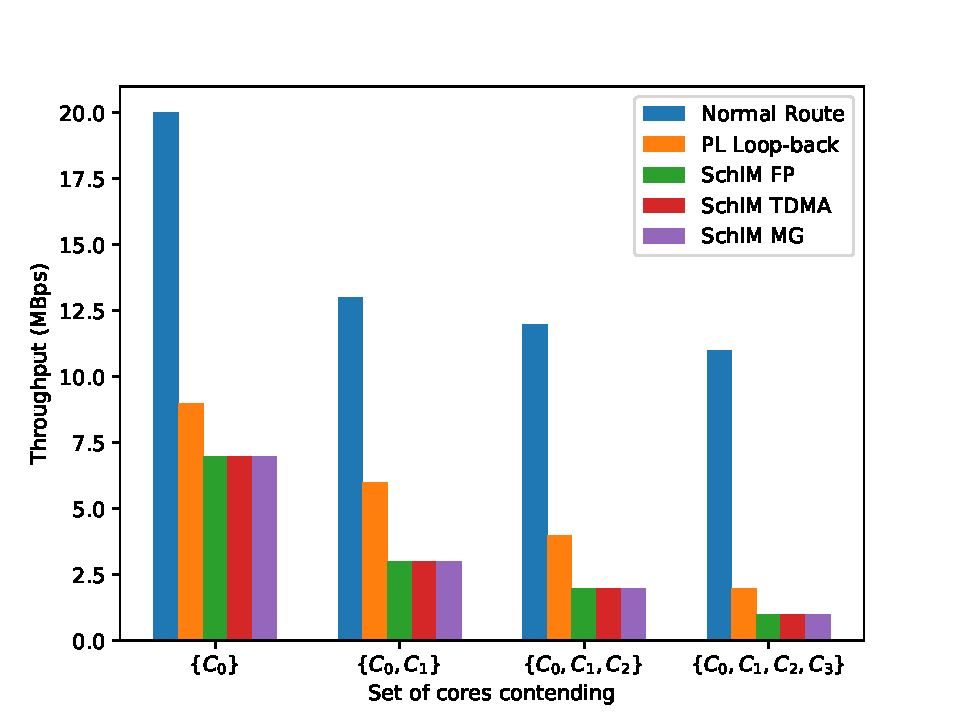
\includegraphics[scale=0.5]{images/bw_comparisons.pdf}
      \caption{Bandwidth in MBps for different path under increasing set of cores contending.}
      \label{fig:bandwidth_comparison}
    \end{figure}

  \subsection{Internal Behaviour of SchIM}
    \label{subsec:internal-behaviour-of-schim}    
    As mentioned earlier, the next objective is to verify the correct behaviour of our scheduling policies at the granularity of a clock cycle by observing the inputs, the outputs and the internal signals and registers of the \schim module.
    This is made possible thanks to the \emph{Integrated Logic Analyser} (or ILA) provided by Xilinx \cite{Xilinx-ILA}. The latter IP can be directly implemented on the PL side, alongside the \schim IP, and is able to probe and signals and to store them in a local memory. For this experiment, the desired signals have been probed and captured during a window of 16384 contiguous clock cycles. Then, the information has been extracted by post-processing the data.
    To characterise the behaviour of the three different policies, the ILA has been used to collect (i) the amount of transactions being buffered in the queues at each clock cycle (subfigure 1 in Figure \ref{fig:schim_behaviour_fp}, \ref{fig:schim_behaviour_tdma}, \ref{fig:schim_behaviour_mg}), (ii) the rate at which queues receive new transactions from the cores cluster (subfigure 2 in Figure \ref{fig:schim_behaviour_fp}, \ref{fig:schim_behaviour_tdma}, \ref{fig:schim_behaviour_mg}) and (iii) the queues ID of each transaction repeated by the \schim module (subfigure 3 in Figure \ref{fig:schim_behaviour_fp}, \ref{fig:schim_behaviour_tdma}, \ref{fig:schim_behaviour_mg}).
    
    For the Fixed Priority trace snapshot displayed in Figure \ref{fig:schim_behaviour_fp}, the following strict priority ordering has been considered: $C_{0} \succ C_{1} \succ C_{2} \succ C_{3}$ where the $\succ$ operator means that the left argument has a strictly higher priority than the right argument. In this experiment, a threshold of 2 for each core has been used.
    As emphasized by the subfigure 2 of Figure \ref{fig:schim_behaviour_fp}, the FP scheduler is able to prioritize the traffic of one core at the expense of the others according to the priorities assignment. Furthermore, one can observe that the rate at which the queues receive new transactions from their associated core is proportional to the priority place in the priority ordering.
    Finally, the third subfigure of Figure \ref{fig:schim_behaviour_fp} confirms the correct behaviour of the FP policy. Thanks to the heat map, one can clearly see that the cores with the highest priority also feature the highest density of transactions at the output of \schim.
    
    The trace snapshot displayed in Figure \ref{fig:schim_behaviour_tdma} has been obtained by configuring the \schim module in TDMA mode. For the sake of clarity, a period of 512 clock cycles have been set for each core. In addition, the threshold of each core has been set to 1.
    The subfigures 2 and 3 of Figure \ref{fig:schim_behaviour_tdma} clearly show the behaviour expected from a TDMA schedule. In fact, one can clearly see in the latter that transactions originating from one core are only being repeated out of the \schim module during a well defined time slot (here, our 512 clock cycles period). Moreover, queues are scheduled one after the other in a periodic fashion.
    In the subfigure 2 of Figure \ref{fig:schim_behaviour_tdma}, we can observe a similar pattern, with transactions arriving only during the TDMA slot associated to their queue (and indirectly core). Globally, the rate at which queues receive transactions is steady and constant. The variations can be explained by different factors such as the coarseness of the FIQ feedback regulation and the scheduling happening on the hypervisor.
    
       The trace snapshot for the TS policy has been obtained with the minimal inter-arrival period set to 256 clock cycles for all the cores. Sinilarly to the TDMA experiment, such period has been set arbitrarily in order to improve the clarity of the trace snapshot displayed in Figure \ref{fig:schim_behaviour_mg}.
       Thanks to the subfigure 3 of Figure \ref{fig:schim_behaviour_mg}, we can see that under an important traffic load, the TS mode of \schim is able to shape the traffic. In the present case, it introduces a minimal time distancing between two transactions originating from a smae core.
       Roughly, the same pattern can be observed in subfigure 2 of Figure \ref{fig:schim_behaviour_mg}. However, there are two exceptions. First, one queue can receive more than one transaction. This is due to the coarseness of the FIQ feedback regulation. Secondly, some queues seem to be prioritized. This can be explained by the fact that in the TS scheduler implementation, ties between valid transactions are resolved by applying a FP policy. In this experiment, the \schim module being constantly under pressure, there are always ties between the queues and FP is always applied.
    \begin{figure}[]
      \centering
      \begin{subfigure}{0.5\textwidth}
        \centering
        % include first image
        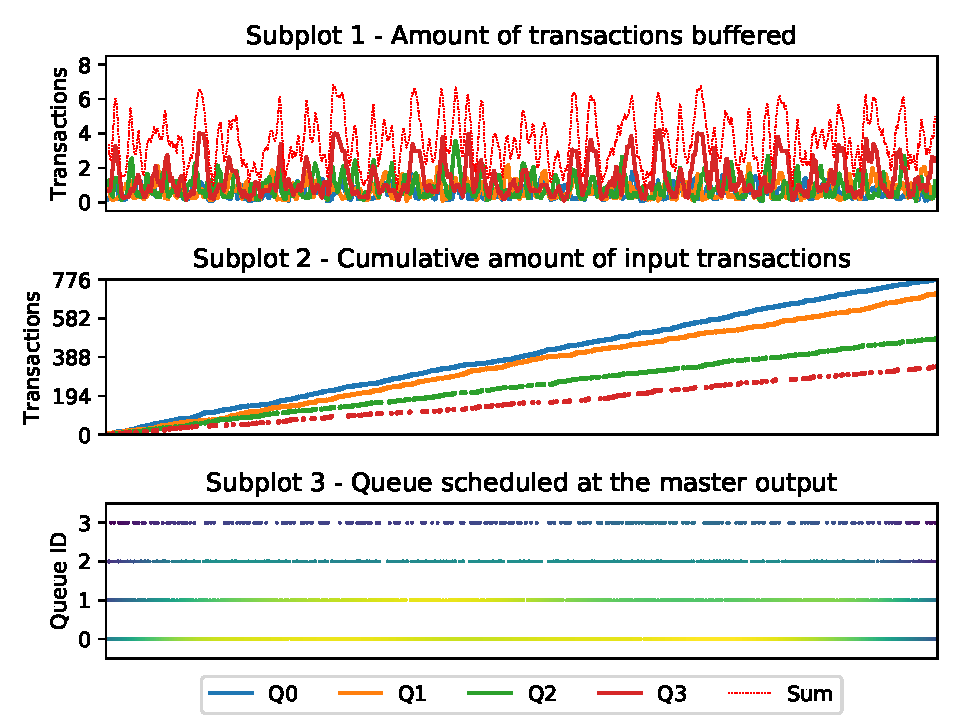
\includegraphics[scale=0.55]{images/SchIM_FP_buffering.pdf}
        \caption{FP with ordering $C_{0} \succ C_{1} \succ C_{2} \succ C_{3}$}
        \label{fig:schim_behaviour_fp}
      \end{subfigure}
      \vfill
      \begin{subfigure}{0.5\textwidth}
        \centering
        % include second image
        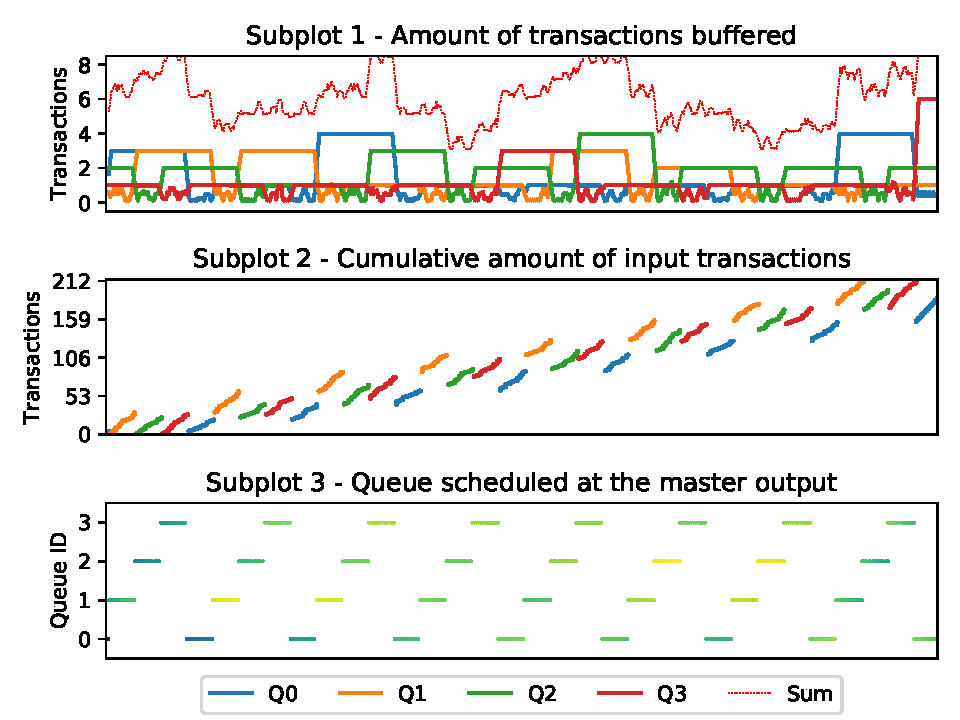
\includegraphics[scale=0.55]{images/SchIM_TDMA_buffering.pdf}
        \caption{TDMA with slots of 512 clock cycles}
        \label{fig:schim_behaviour_tdma}
      \end{subfigure}
      \vfill
      \begin{subfigure}{0.5\textwidth}
        \centering
        % include second image
        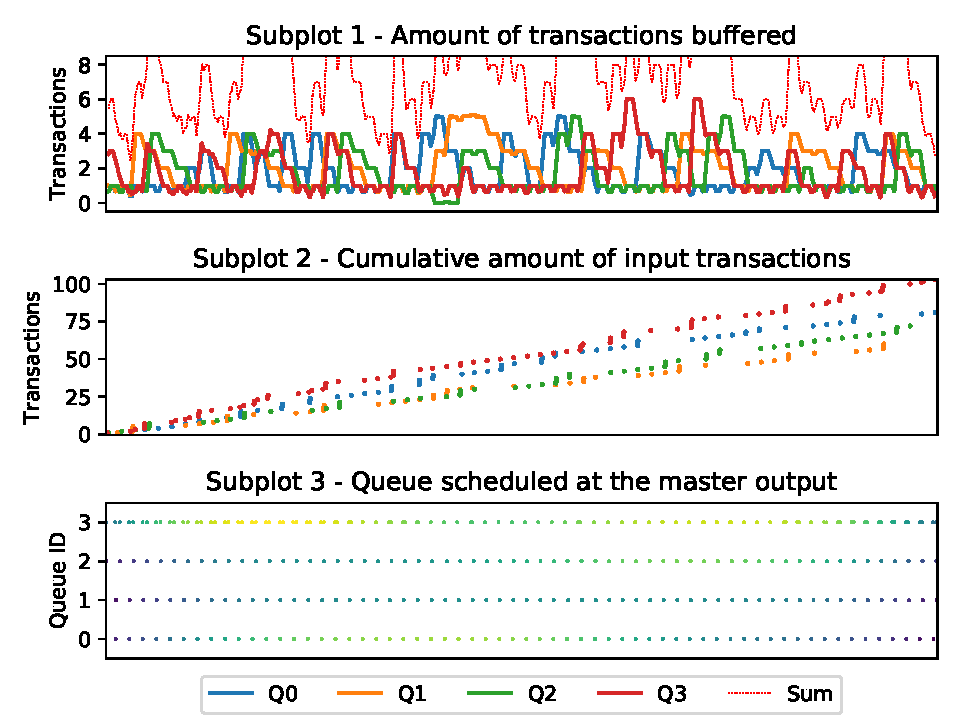
\includegraphics[scale=0.55]{images/SchIM_MG_buffering.pdf}
        \caption{TS with min. period of 256 clock cycles}
        \label{fig:schim_behaviour_mg}
      \end{subfigure}
      \caption{Trace snapshots of SchIM for FP (\ref{fig:schim_behaviour_fp}), TDMA (\ref{fig:schim_behaviour_tdma}) and TS (\ref{fig:schim_behaviour_mg})}
      \label{fig:schim_behaviour}
    \end{figure}

  \subsection{Memory Isolation}
    To evaluate the capability of \schim to ensure the memory isolation of the cores, an experiment consisting in comparing the execution time of one core when running one benchmark alone (also referred to as \emph{Solo}) and when running alongside memory bombs (also referred to as \emph{Stressed}). The ratio of the latter and the former indicates whether (and to which extent) the execution time of the benchmark suffered from inter-core interferences. Typically, a ratio of 1 denotes a perfect isolation. The benchmarks listed in Table \ref{tab:isolation_ratio} have been chosen as their are \emph{Memory Bound}.
    
    The Loop-back path is used as a baseline for this experiment. Its ratios, displayed in the left most column of Table \ref{tab:isolation_ratio}, highlight the sensitivity of both disparity and mser benchmarks to inter-core interferences, with ratios of respectively $1.46$ and $1.59$. On the other hand, texture synthesis and localization naturally do not suffer from inter-core interference. In comparison, the TDMA scheduler manages to guarantee the isolation of the core under analysis. In fact, the ratio of all the benchmark tested lie in the vicinity of 1.0, with a maximum inter-core interference of 7\%. Similarly, the TS scheduler is also capable of ensuring a sound isolation of the core under analysis. Unfortunately, the FP scheduler is unable to guarantee the isolation of the core under analysis despite having been assigned the highest priority. Even worst, the scheduler has no or little impact as its ratios are similar to the ones of the loop-back path.
    This result can be explained by the fact that despite the effort of the FP scheduler and its proven correct behaviour (see Figure \ref{fig:schim_behaviour_fp}), the enforced ordering of transaction is being overridden by the mechanisms present in the DDR controller. The FP scheduler works perfectly in scenarios like Figure \ref{fig:schim_behaviour_fp} because the transactions are sequential whereas, it is not always the case for real application. In consequence, the FP module is mainly useful in the case of big data movements.
    \begin{table}[]
      \centering
      \caption{Inter-core Interference Ratios}
      \label{tab:isolation_ratio}
      \begin{tabular}{|c||c|c|c|c|}
      \hline
      \multirow{2}{*}{Benchmark} & \multicolumn{4}{c|}{Paths}                          \\ \cline{2-5} 
                                 & Loop-back & \schim TDMA & \schim TS & \schim FP \\ \hline\hline
      stitch                     & $1.14$    & $1.06$      & $0.98$    & $1.16$    \\ \hline
      texture synth.             & $1.03$    & $1.02$      & $1.0$     & $1.03$    \\ \hline
      disparity                  & $1.46$    & $1.07$      & $0.96$    & $1.46$    \\ \hline
      tracking                   & $1.13$    & $1.05$      & $0.97$    & $1.13$    \\ \hline
      localization               & $1.02$    & $1.01$      & $1.0$     & $1.02$    \\ \hline
      mser                       & $1.59$    & $1.06$      & $0.98$    & $1.56$    \\ \hline
      sift                       & $1.14$    & $1.04$      & $0.97$    & $1.14$    \\ \hline
      \end{tabular}
    \end{table}
